%Master document for paper.
%Created MS 4/12

\documentclass[12pt,notitlepage]{article}

\usepackage[text={6.5in,9in},centering]{geometry}               % See geometry.pdf to learn the layout options. There are lots.
\geometry{letterpaper}                   % ... or a4paper or a5paper or ... 
%\geometry{landscape}                % Activate for for rotated page geometry
\usepackage[parfill]{parskip}    % Activate to begin paragraphs with an empty line rather than an indent
\usepackage{subfigure}
\usepackage{graphicx}
\usepackage{setspace}
\usepackage{color}
\usepackage{amssymb}
\usepackage{amsmath}
\usepackage{listings}
\usepackage{epstopdf}
\usepackage{epsfig}
%\usepackage{psfig}
\usepackage[dvips, bookmarks, colorlinks=true, linkcolor=blue, citecolor=blue, pdftitle={Investigation of the Properties of Superfluid He4}, pdfauthor={Baryakhtar, Schowalter, Swiatlowski}, pdfsubject={Physics 191 Lab Report}, pdfkeywords={helium, superfluid, physics, 191}]{hyperref}
\DeclareGraphicsRule{.tif}{png}{.png}{`convert #1 `dirname #1`/`basename #1 .tif`.png}
\usepackage{cite}

\begin{document}

%\title{Investigation of the Properties of Superfluid He$^4$}
%\author{Maria Baryakhtar \footnote{Produced Introduction and
%    Background (Sections \ref{introduction}, \ref{background}),
%    Appendix ~\ref{masscalibration}, and Abstract} \and Steven
%  Schowalter \footnote{Produced Results and Discussion (Section
%    \ref{resultsanddiscussion}) and Appendix
%    ~\ref{muontimeerroranalysis}} \and Maximilian Swiatlowski
%  \footnote{Produced Instrumentation and Procedure (Sections
%    \ref{instrumentation}, \ref{procedure})}}

%\maketitle
%\thispagestyle{empty}

\begin{titlepage}
\begin{center}

\ \\
\vspace{1in}

{\Huge
Investigation of the Properties of the Rubidium Atomic System with Optical Pumping Methods
\\}
\ \\

%\large{In partial fulfillment of the requirements of Physics 191r at Harvard University}

Maria Baryakhtar \footnote{Harvard University, Cambridge MA 02138 \\ \qquad \qquad Masha Baryakhtar produced the Background~(\ref{background}) and Conclusion~(\ref{conclusion}) sections, and the superfluid fraction calculation~(\ref{superfluiddensity}). \\ \qquad Steven Schowalter produced the Results~(\ref{results}) and Analysis~(\ref{analysis}) sections and the Appendices. \\ \qquad Maximilian Swiatlowski produced the Abstract, Introduction~(\ref{introduction}), and Experimental~(\ref{experimental}) sections.}, Steven Schowalter \footnotemark[\value{footnote}], Maximilian Swiatlowski \footnotemark[\value{footnote}] 

\ \\

%Abstract body
%Created MS 05-11

\end{center}

\begin{abstract}
% put text of the abstract here 

We present measurements and observations of several properties of optically pumped rubidium atoms. A vapor of mixed $^{85}$Rb and $^{87}$Rb is brought to a preferential $m_{F}$ state through absorption of circularly polarized light. The g-factors of the two isotopes are measured by coupling the system to radiofrequency magnetic field and finding the strongest coupling frequency. The optical pumping time $\tau$ and spin relaxation time $T_{1}$ are measured by optically pumping the system and then letting it evolve without light for variable periods of time. The spin decoherence time $T_{2}$ and related power-broadening effects are measured as functions of the intensity of light and radiofrequency amplitude. Finally, we find the spin-exchange rate between the two isotopes by pumping one and driving Rabi oscillations on the other. The g-factors are calculated to be $g_{f}=0.30\pm0.03$ for $^{85}$Rb and $g_{f}=0.46\pm0.05$ for $^{87}$Rb, in very good agreement with predicted values $g_{f}=0.33$ and $g_{f}=0.50$ respectively. Times for optical pumping and spin relaxation are reasonable, and $T_{2}$ displays the expected power-broadening behavior. The calculated spin-exchange rates are in good agreement with the understanding that most of the spin decoherence rate is due to spin-exchange collisions. 

\end{abstract}
\begin{center}

%; ratio $1.5\pm0.2$


\end{center}
\end{titlepage}

\clearpage

%Introduction body
%Created MB 04-12

\section{Introduction}\label{introduction}

Optical pumping is the process in which atoms are populated using circularly polarized light to a preferred magnetic sublevel, split from degeneracy using the Zeeman effect. A number of unique quantum properties are observed when an ensemble of atoms are in a single spin projection state. The range of experiments available which utilize optical pumping, usually related to radiofrequency spectroscopy \cite{bloom}, are therefore very wide, with topics ranging from measurement of the g-factors of different atoms and the electron to analysis of the functional form of power-broadening and spin-alignment decay rates.

Our experiment consists of several different measurements, most of which can be compared to analytically derived expected forms. First, general measurements of the effectiveness of the optical pumping, the properties of the transient behavior, and the behavior of Rabi oscillations are performed. By stepping across different radiofrequencies applied to the system and measuring the root mean square amplitude of the Rabi oscillations, we are able to find the frequency corresponding to the Zeeman energy splitting of the atoms and therefore calculate the g-factors $g_{F}$. Then, it is possible to measure the natural decay time $T_{1}$ of the metastable spin state by letting the system evolve without the presence of the optical pumping laser. Next, we measure the time constant $T_{2}$ associated with the natural spin decoherence rate of the spin projections by measuring the linewidth of the Rabi oscillation amplitudes as a function of frequency. Finally, we are able to measure the spin-exchange rate between $^{85}$Rb and $^{87}$Rb by analyzing the Rabi oscillations when pumping one isotope and driving the other with an oscillating magnetic field.

In Section~\ref{background}, \emph{Background}, we introduce the theoretical basis for optical pumping, the qualities of the rubidium atom which make it ideal for pumping and Rabi oscillations. We derive the approximate analytic expressions for the power-broadening behavior of the linewidths $\gamma_{1}$ and $\gamma_{2}$ by solving a system of simplified 2 and 3 state rate equations. In Section~\ref{experimental}, \emph{Experimental}, we describe the various experimental techniques used in the experiment, including methods used to generate magnetic fields and the optics. Raw data accumulated from the experiments is presented in Section~\ref{results}, \emph{Results}. The algorithms used to process the data and the calculated values, as well as errors, are given in Section~\ref{analysis}, \emph{Analysis}. Finally, the results are summarized and compared to expected forms, and experimental improvements are suggested in Section~\ref{conclusion}, \emph{Conclusion}.

%Background body
%Created MS 05-11

\section{Background}\label{background}

\subsection{Optical Pumping}

Optical pumping is the process in which the interaction of light with
atoms produces a population of energy levels that is distinct from the
thermal equilibrium Boltzmann distribution \cite{bernheim}.

In this experiment, we consider a Rubidium atom and focus on the $D_1$
transition between the $^2P_{1/2}$ and $^2P_{3/2}$ excited states.

\subsection{Rubidium System}

\subsubsection{$^{85}$Rb and $^{87}$Rb levels}

\subsection{Magnetic Interactions}

\subsubsection{Zeeman Splitting}

\subsubsection{Rabi Oscillations}

\subsection{Rate Equations}


\subsection{Spin Exchange}

%Experimental body
%Created MB 04-12

\section{Experimental}\label{experimental}

\subsection{Apparatus}\label{apparatus}

The goal of the experimental apparatus is to create a robust system in which atoms can interact with electromagnetic fields in a controlled fashion. A glass cell containing rubidium metal and chosen buffer and exchange gases \footnote{Our experiment was run with $1.43$ cm of N$_{14}$ and $34.99$ cm of He as exchange and buffer gasses respectively, where cm is displacement of oil, density $0.906$ g/cm$^{3}$. The volume of the cell was $300$ cm$^{3}$.} is placed into a cylindrical mu-metal shell with openings at the ends, which serves to shield the experiment from the earth's magnetic field. Inside the cylinder, a resistive element is used as a heater and a Hewlett Packard platinum film thermometer monitors temperature, providing a fairly accurate temperature control system. \footnote{As the thermometer is slightly magnetic, it is important to remove it before taking measurements.} The experiment is generally operated at $49.6\pm0.3^{\circ}$ C. A $12$'' diameter, $27.75$'' long aluminum cylinder inside the shield is wound with $1064\pm4$ turns of enameled wire, creating a uniform magnetic field inside the solenoid. The electromagnet is supplied with current from a set of $6$ C cell batteries, for a combined $9$ V, while a potentiometer allows for control of the current in the range of $5$ to $50$ mA and a $1 \Omega$ series resistor allows for accurate monitoring of the solenoid current. \footnote{Note that the current from the batteries drifts downwards over time, and while great care was taken to ensure a constant magnetic field, ultimately the measurement of the current may vary by as much as $0.03$ mA.} Finally, the shield also houses a set of Helmholtz coils which, when driven by a function generator, will provide the radiofrequency fields for the atoms. The glass cell is placed directly in the center of the Helmholtz coil, allowing for a rather uniform distribution of the field through the pumping region.

The optics of the experiment are set up as in Fig.~\ref{fig:optics1} below.

\begin{figure}[htbp]
\begin{center}
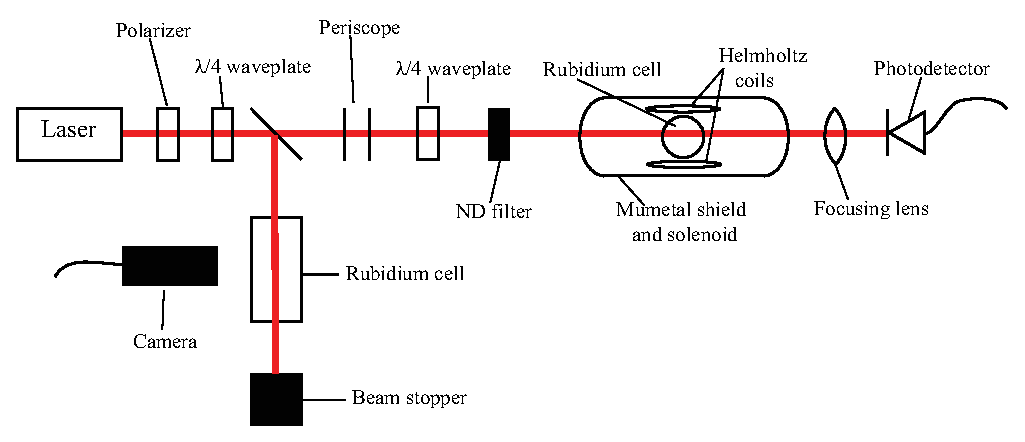
\includegraphics[width=6.5in]{./figures/optics1.eps}
\caption{\small{The generic optics arrangement used in this experiment.}}
\label{fig:optics1}
\end{center}
\end{figure}


The laser used in the experiment is a Sharp LT025MD tunable laser diode with grating feedback. Because wavelength increases as a function of temperature and the free-running wavelength of the laser is only $790$ nm and the D1 wavelength is $794$ nm, the laser is operated at approximately $50^{\circ}$ C. A system of thermoelectric coolers and a more fine-tuned temperature control circuit keep the temperature of the laser steady in order to maintain wavelength stability. Adjusting the current supplied to the laser allows for fine control of the wavelength and power of the laser. Note that there is no independent power and wavelength control; furthermore, the laser current drifts down over time. However, as the laser did not drift out of the sensitive region of the rubidium during any of the experiments, this had little effect upon the measurements. Upon leaving the laser housing, the beam is both collimated and linearly polarized.

The next piece of optics the laser encounters is a linear polarizer and a quarter wave plate cemented to the face of a polarizing cube. This combination is used to prevent back reflection into the laser; furthermore, the circularly polarized light will be split $50-50$ by the polarizing beam-splitter cube. 

The diverted beam shines through a small cylinder filled with rubidium vapor before ending at a beam-stopper. A small plastic housing encloses the cylinder and allows an infrared camera to monitor the fluorescence of the rubidium as the laser passes through. By adjusting the laser current and monitoring the fluorescence on a television attached to the camera, it is possible to accurately set the laser to the desired rubidium transition line.

The other part of the beam first is raised by a periscope to bring it into the plane of the shielding cylinder. After leaving the beam splitter the laser light is once again linearly polarized, so a quarter wave plate is used to circularly polarize it. The light then encounters an optional neutral density (ND) filter and passes through the cylinder and the rubidium cell; depending upon the magnetic fields present, portions of the laser light will be absorbed. After the beam leaves the cylinder, a lens with a $100$ mm focal length focuses it onto a variable-gain Thorlabs PDA36A photodetector. \footnote{Note that the photodetector is mounted with an $800$ nm interference filter, which enables the experiment to be run with the room lights on and guaranteeing that any light detected is in the neighborhood of the appropriate wavelength.} The signal from the photodetector, which is able to distinguish the varying degrees of absorption in the rubidium, is then read by a voltmeter or an oscilloscope. Optical pumping is detected by the transition of atoms into the dark state, where they are unable to absorb the circularly polarized light. This increases the transmission of the laser through the gas, and the photodetector signal rises.

%probably want to cut most of this section.
%The general system of optical pumping that we observe works as follows: circularly polarized light interacts with the rubidium atoms, and some of them absorb the photons and enter the excited state with $l_{e}=l_{g}+1$ (the sign depending on the polarization direction of the light, but chosen here to be positive for simplicity). The excited atom will spontaneously decay down to any allowed ground state, \emph{i.e.} $l_{g} = l_{e} \pm 1$. However, the atoms in the most extreme $+l$ state will not be able to be transferred to the excited state, as there is no way for them to increase their $l$. As atoms decay from the excited state into allowed ground states equally, the ones that fall into $l=l-1$ will be moved back to the excited state until they decay again. Each time this decay occurs, half the atoms move into the extreme state, and so eventually all the atoms will be in this state. Experimentally, this is observable as an increase in the transmission of the laser through the atoms, as the light is not absorbed when the atoms are in the extreme, ``dark'' state. 

\subsection{Direct Signal Measurements}\label{directsignalmeasurements}

The goal of the first group of experiments was to determine the transient behavior of the atoms as the solenoid field is turned on and off, and to understand the Rabi oscillations present when the radiofrequency magnetic field is applied. The current applied to the solenoid was $19.93$ mA.

The study of the transient behavior was performed by first tuning the laser to the appropriate transition and setting the oscilloscope trigger level appropriately. As the solenoid magnetic field is turned on, the magnetic sublevels of the atom split and optical pumping becomes possible. Transmission of the laser goes up as more atoms are put into a dark state that cannot absorb the circularly polarized light. By studying the oscilloscope trace, it is possible to estimate the optical pumping time associated with the atoms and the given light intensity. Furthermore, by studying the decay of the signal after the magnetic field is turned off, it is possible to estimate the relaxation time of the atoms' spin, $T_{1}$. Both of these measurements are approximate at best, because of the finite rise and fall times associated with the inductance of the magnet. \footnote{More complete measurements are described in Section \ref{measurementoft1}.} However, because of the simple procedure, the data is still worth taking and comparing to more correct measurements. Moreover, this procedure provides a simple measurement of the strength of the optical pumping the system is able to achieve by comparing the magnitudes of the on and off states.

To study the Rabi oscillations, the function generator was set to create a radiofrequency wave at hundreds of kHz. \footnote{The exact frequency was chosen from calculated values of $g$ factors and the Zeeman splitting, as in Section~SOMETHING} The signal was amplitude modulated from $0$ to $100\%$ at a frequency of $21$ Hz, slow enough to allow the Rabi oscillations to settle into a steady state. We set the oscilloscope to trigger on the frequency generator's sync signal and to time average over repeated cycles so as to minimize noise. All data was taken on a Textronix TD3812 oscilloscope.

\subsection{Measurement of $T_{1}$}\label{measurementoft1}

To measure $T_{1}$ more accurately, it would be ideal to turn off the optical pumping laser instantaneously, let the atoms evolve in the dark for a chosen time period, and then measure the transmission of the laser through the atoms. As the atom spins decay to a thermal distribution, more atoms will be able to absorb the circularly polarized light, and transmission of the laser will decrease. As the laser optically pumps the atoms, the transmission will once again increase, but at the instant that the laser is applied, the transmission level provides accurate information about the distribution of the dark state of the atoms. Furthermore, the rise of the transmission will provide an accurate measurement of the optical pumping rate of the atoms. The question, then, is how to instantaneously turn off the laser for variable lengths of time.

The solution is a Stanford Research Systems SR540 optical chopper. By placing the chopper in the middle of the beam as in Fig.~\ref{fig:optics2} it is possible to regularly turn on/off the beam at a chosen frequency. However, as the beam is rather wide when it leaves the laser, it is necessary to use a series of $50$ mm focal length lenses to focus the beam at the chopper and then expand it back to size: otherwise, the chopping time would be finite and not instantaneous, as the beam would be slowly covered by the surface of the chopper. \footnote{The beam is re-expanded so as to be able to interact with a larger cross-section of atoms in the glass cell.} The signal from the photodetector is monitored on an oscilloscope and analyzed as discussed above. At higher chopping frequencies, it is possible to trigger and time average on the oscilloscope, reducing signal to noise. \footnote{The averaging is not possible to perform at lower frequencies, as the chopper is very slightly damaged and does not spin perfectly evenly. This effect is only visible at lower frequencies, as at higher frequencies the chopper spins so quickly that the uneven portion is exposed for very short periods of time.}


\begin{figure}[htbp]
\begin{center}
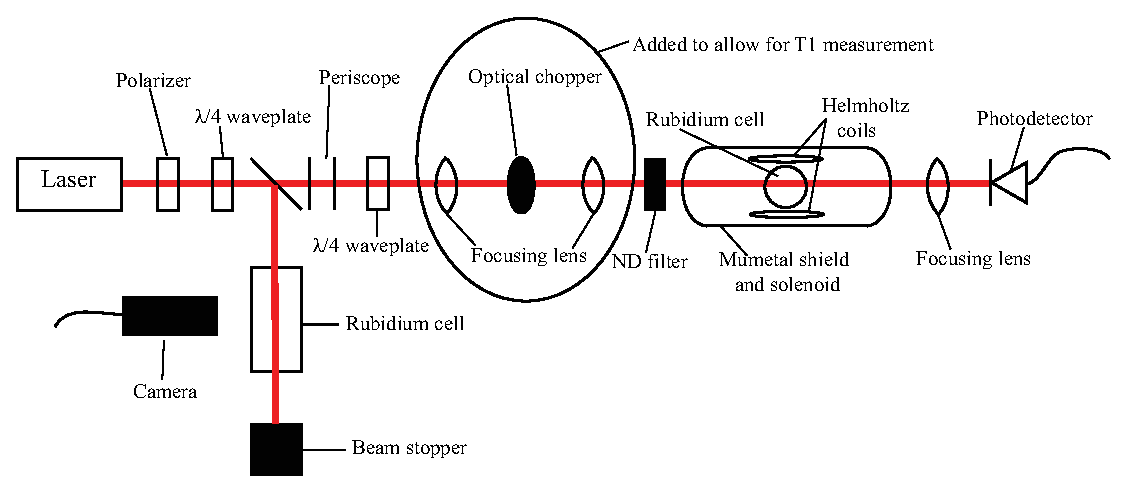
\includegraphics[width=6.5in]{./figures/optics2.eps}
\caption{\small{The modified optics arrangement used to measure $T_{1}$. Note the addition of the $50$ mm lenses on either side of the optical chopper.}}
\label{fig:optics2}
\end{center}
\end{figure}


Note that at higher frequencies, the signal will be chopped before the atoms have reached the completely pumped state, and so the transmission level they start from will be lower than the true equilibrium seen at lower frequencies. To normalize, both the level of transmission before the dark period and after are measured and the ratios at different frequencies are compared. As the decay is exponential, it always occurs at the same rate and so the ratios are enough to calculate the decay constant. The measurements were all performed on the $3\rightarrow3$ $^{85}$Rb transition, as the $^{87}$Rb value is much more difficult to measure because of the lower concentration of this isotope in the cells we used.

\subsection{Measurement of $T_{2}$} \label{measurementoft2}

To gain a better understanding of the properties of the atom, it is also desirable to measure the $T_{2}$ of the atom: \emph{i.e.} the time constant associated with the rate at which the atomic spins lose coherence. As derived in section SOMETHING, the linewidth of the Lorentzian is inversely proportional to the $T_{2}$ time of the atoms. The principal experimental difficulty is the power-broadening of the linewidth at high radiofrequency signals and high laser intensities. In the limits where only one broadening factor contribute, we have as derived in sections BLAH and BLAH, we have:

\begin{eqnarray}
\gamma_{m} &=& \gamma \sqrt{1+ \kappa_{rf} B^{2}} \label{eq:rfbroad}\\
\gamma_{m} &=&\gamma \sqrt{1+ \kappa_{las} \mathcal{E}_{0}^{2}} \label{eq:lightbroad}
\end{eqnarray}

where $\gamma_{m}$ is the measured linewidth, $\gamma$ is the real linewidth, $B$ is the amplitude of the radiofrequency fields, $\mathcal{E}_{0}^{2}$ is the intensity of the laser, and the $\kappa$ factors are constants. Combining the equations is a complicated matter which requires a full derivation of the three-state system, so we consider the effects separately by measuring them in the limits where the other factor does not contribute greatly. The goal, then, is to measure the linewidth as independent functions of radiofrequency amplitude and light intensity and extrapolate both back to the asymptotic region where the broadening factor does not contribute.

To measure the linewidth, we record the amplitude of the the Rabi oscillations at different rf frequencies, with the rf signal chopped as described in Section \ref{directsignalmeasurements}. To increase signal to noise when measuring this amplitude, a lock-in amplifier is synced to the function generator, and the resulting signal is read by a voltmeter. A LabView program interfacing with the function generator and the voltmeter steps through different frequency settings and records the amplitude after a given averaging time.

To find the function dependent on rf amplitude, we insert a strong ND $2.0$ filter so as to remove SOME $\%$ of the light. \footnote{We guessed that this would be low enough intensity that the signal was not broadened; later results proved this correct, but if they hadn't, we would have repeated this experiment with a higher strength ND filter.} The LabView program can also control the peak-to-peak voltage of the function generator, allowing the linewidth to be recorded at many different voltage levels. This data is fit to Eqn. \ref{eq:rfbroad}, allowing for $\gamma$ to be calculated. Note that between measurements it is important to realign the laser to the appropriate transition, as the laser tends to drift slightly off over long periods of time. This has little effect on actual data runs, but would compound over multiple measurements.

The procedure for measuring the dependence on the light intensity is very similar. From the fit above, a value of the radiofrequency amplitude low enough to be in the asymptotic region is selected. Then, the ND filter is adjusted in increments of $0.1$ and the linewidth recorded using the LabView program. The resulting linewidths are fit to Eqn. \ref{eq:lightbroad} and extrapolated to 0 intensity.  Note that this plot confirms that an ND value of $2.0$ is in the asymptotic region, so our selection in the original experiment was acceptable.

This procedure was performed on the $3\rightarrow3$ transition in $^{85}$Rb. The rf measurement was also performed with an ND of $2.0$ (again, sufficiently high to be safe) on the $2\rightarrow2$ transition in $^{87}$Rb. Thus, we were able to measure the $T_{2}$ time for both isotopes of rubidium. Whereas the difference between $T_{1}$'s is not particularly interesting and was therefore omitted, the difference here is related to the different spin-exchange rates of the two isotopes.

\subsection{Measurement of $^{85}$Rb and $^{87}$Rb Spin-Exchange Rate}

One of the factors contributing to the $T_{2}$ relaxation time are spin-exchange collisions between the different gasses in the cell. It is possible to measure this rate by shining the laser on say, a $^{85}$Rb transition, and driving the radiofrequency at the $^{87}$Rb rate. The $^{87}$Rb will be undergoing Rabi oscillations and will transfer their spins to the $^{85}$Rb at each point of the oscillation, as discussed in section BLAH. Because of these spin exchanges, the $^{85}$Rb will be effectively undergoing Rabi oscillations, and we should be able to measure the normal Lorentzian distribution at around the $^{87}$Rb rf frequencies, even though the $^{87}$Rb is not being optically pumped. The linewidth here will correspond, just as in previous experiments, with a power-broadened natural linewidth:

\begin{equation}
\gamma_{m} = \gamma_{se} \sqrt{1+\kappa_{rf} B^{2}} \label{eq:sebroad}
\end{equation}

The resonance of the $^{85}$Rb at the frequencies which correspond to $^{87}$Rb can be due to only the spin-exchange mechanism, so it is natural to call the unbroadened linewidth $\gamma_{se}$, the spin-exchange rate. Furthermore, we expect power-broadening of the same rf form as we've seen before: a larger rf amplitude will increase the rate of coupling, and there should still be coupling with no radiofrequency field. Note that because of the different concentrations of rubidium isotopes, the spin-exchange rates will not be symmetric; \emph{i.e.}, because there is little  $^{87}$Rb, driving this frequency will have a very small effect on the $^{85}$Rb, whereas driving on the  $^{85}$Rb rf frequencies will have a much larger effect on the  $^{87}$Rb.

Experimentally, the primary obstacle in this measurement is this very low strength of the coupling and therefore the very low amplitude of the measured oscillations. To compensate, the sensitivity of the lock-in amplifier is set to $20 \mu$V here, up from $5$ mV in the previous experiments. A 2.0 ND filter ensures that there is no power-broadening due to light, and measurements are performed using the LabView program at different radiofrequency amplitudes. The data is fit to Eqn. \ref{eq:sebroad} and extrapolated to 0 amplitude, allowing for a calculation of $\gamma_{se}$. The measurement is performed on the $3\rightarrow3$  $^{85}$Rb transition and the $2\rightarrow2$ $^{85}$Rb transition. 

\subsection{Measurement of Rubidium $g$-factor}

As discussed in Section BLAH, the peak of the Rabi oscillation amplitudes occurs at the frequency corresponding to the Zeeman splitting of the magnetic sublevels. By measuring this frequency and calculating the magnetic field of the solenoid, it is possible to calculate the $g$-factor of the atom, according to equation SO AND SO.

The calculation of the magnetic field is straightforward when the solenoid properties and current are known. To measure the peak frequency, the LabView program is used to produce the spectrum at several different radiofrequency amplitudes. The maximum frequency should not move because of power-broadening, so the center of these curves are averaged and this value is chosen as the splitting frequency. This measurement is performed on all of the available rubidium splittings.














%Results body
%Created SS 04-14

\section{Results}\label{results}

\subsection{Observing Optical Pumping and RF Coupling}\label{ObservingOpticalPumpingandRFCoupling}

With the external magnetic field applied, laser light is used to optically pump rubidium atoms into a preferential spin state.  To observe this pumping, we measure the transmission of laser light through the cell using a photodetector.  Transmission will increase when atoms are optically pumped into an excited $m_F$ state and no longer absorb the laser light. This sample data is observed on an oscilloscope as shown in Fig. \ref{fig:raw_data}.
\begin{figure}[htbp]
\begin{center}
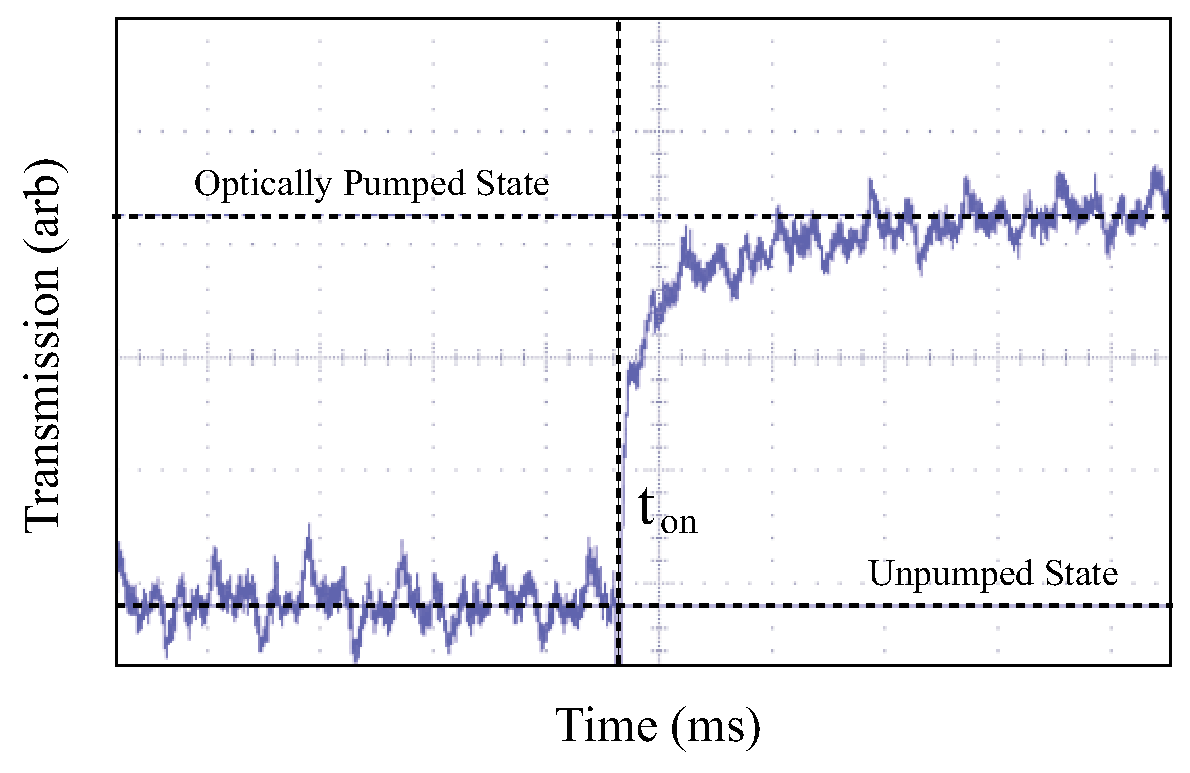
\includegraphics[height=70mm]{./figures/raw_data.eps}
\caption{\small{Sample oscilloscope data of optical pumping. At $t=t_{on}$, the external magnetic field is turned on. The subsequent Zeeman splitting enables the rubidium atoms to be optically pumped to preferential $m_F$ state using laser light.  Optical pumping is observed in the increase of transmission to a higher steady state level.}}
\label{fig:raw_data}
\end{center}
\end{figure}
A radiofrequency magnetic field is used to disrupt the optically pumped steady state by coupling the pumped $m_F$ state to the next (lower) $m_F$ state.  This coupling creates a transient phenomenon which is characterized by the decrease in signal from the pumped level to some new steady state.  In order to closely analyze the transient portion due RF interference, a chopped RF signal is used.  
\begin{figure}[htbp]
\begin{center}
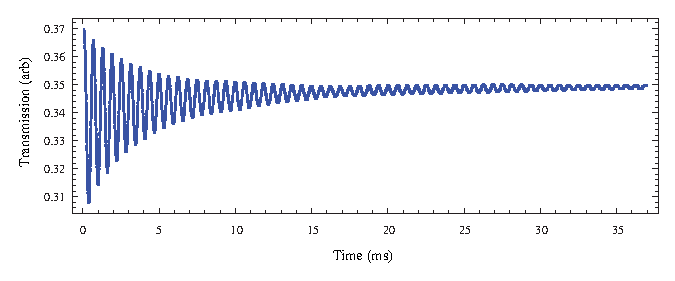
\includegraphics[height=70mm]{./figures/rabi.eps}
\caption{\small{Rabi oscillations resulting from radiofrequency coupling of $m_F$ states while optically pumping $^{85}$Rb.}}
\label{fig:rabi}
\end{center}
\end{figure}
The depumping caused by the $m_F$ coupling combined with optical pumping creates Rabi oscillations in the transient portion between the fully state and the new equilibrium.  This phenomenon is shown in Fig. \ref{fig:rabi}.  The oscillations signify periodic fluctuations in spin state populations due to the $m_F$ coupling, as predicted by Eqn.~\ref{eqn:rabi}.

\subsection{Measuring Linewidth and Optical Pumping Resonance}\label{MeasuringLinewidthandOpticalPumpingResonance}

Using a lock-in amplifier, we measure the amplitude of Rabi oscillations as a function of the applied radiofrequency.  We use a LabView program in order to select and step through a range of radiofrequencies in order to observe the Lorentzian resonance.  This data was taken for both $^{85}$Rb and $^{87}$Rb. This data is shown in Fig. \ref{fig:rawcurve}.    
\begin{figure}[h!]
\begin{center}
\subfigure[$^{85}$Rb ($3\rightarrow3$)]{\label{fig:edge-a}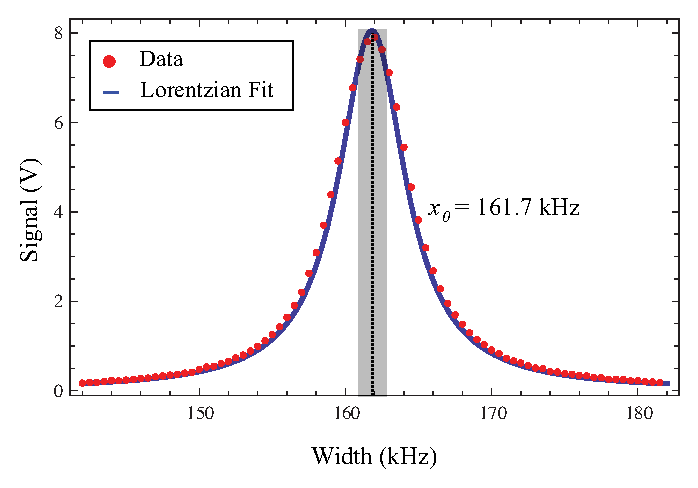
\includegraphics[height=50mm]{./figures/85raw_width.eps}}
\hspace{-1mm}
\vspace{-2mm}
\subfigure[$^{87}$Rb ($2\rightarrow2$)]{\label{fig:edge-b}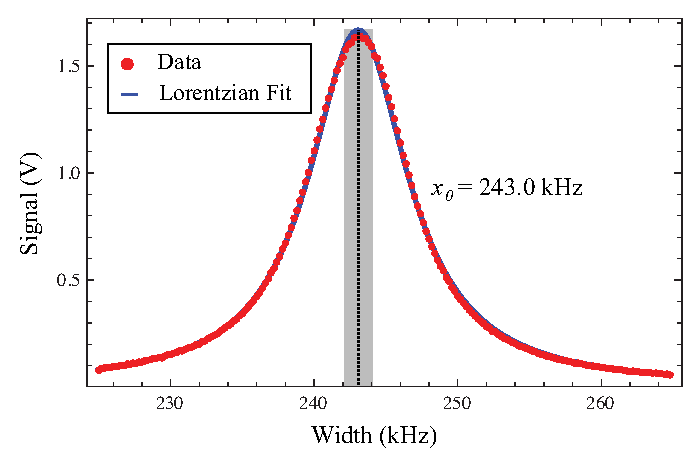
\includegraphics[height=50mm]{./figures/87raw_width.eps}}
\vspace{-2mm}
\caption{\small{Optical pumping resonances for rubidium isotopes. Fitting this data to Lorentzian distributions, we are able to determine the resonant frequencies at which $m_F$ states couple. For $^{85}$Rb and $^{87}$Rb, these resonant frequencies are $161.0 \pm 0.8$ kHz and $243.1\pm 0.3$ kHz respectively. We are also able to use this data to measures the linewidth.}}
\label{fig:rawcurve}
\end{center}
\end{figure}
This data was fit to Lorentzian distributions. These fits were then used to calculate the resonant frequencies.  The resonant $m_F$ coupling frequencies for $^{85}$Rb and $^{87}$Rb are $161.0 \pm 0.8$ kHz and $243.1\pm 0.3$ kHz respectively.  

Further measurements are taken using the $^{85}$Rb $3\rightarrow3$ transition to determine the effect of radiofrequency amplitude and laser light intensity on the linewidth of the resonance. By independently varying either of these variables, several resonances are measured.  Using a \emph{Mathematica} program, the linewidths of these resonances are calculated and plotted with respect to both radiofrequency amplitude and laser light intensity.  This data is shown in Fig. \ref{fig:linewidths}.
\begin{figure}[h!]
\begin{center}
\subfigure[Varying RF Amplitude]{\label{fig:edge-a}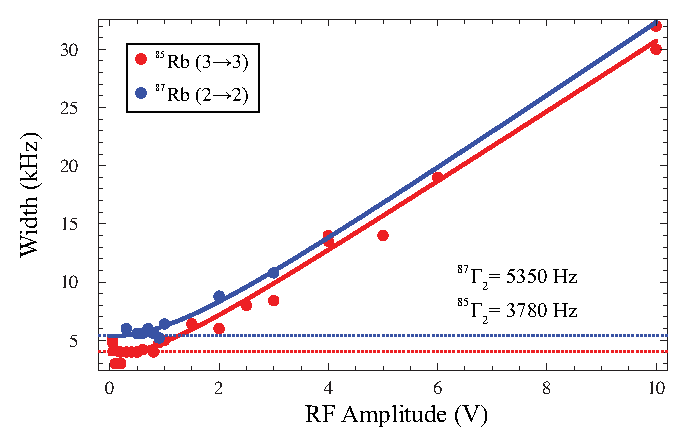
\includegraphics[height=50mm]{./figures/amp_width.eps}}
\hspace{-1mm}
\vspace{-2mm}
\subfigure[Varying Intensity]{\label{fig:edge-b}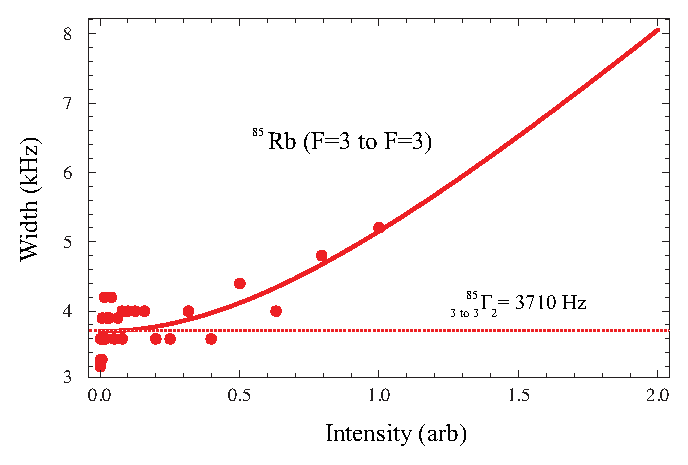
\includegraphics[height=50mm]{./figures/intensity_width.eps}}
\vspace{-2mm}
\caption{\small{Power broadening of rubidium linewidths due to laser light intensity and RF amplitude.  The data in (a) is fit to $\alpha \sqrt{1+\beta x^2}$ whereas the the data in (b) is fit to $\alpha \sqrt{1+\beta x}$.  With these fits we are able to determine the natural $\gamma_2$ linewidths for $^{85}$Rb and $^{87}$Rb which are found to be $3.70 \pm 0.48$ kHz and $5.35 \pm 0.47$ kHz respectively.  Error is either identified by the thickness of the points (a) or error bars (b).}}\label{fig:linewidths}
\end{center}
\end{figure}
The variable being held constant was chosen in a regime in which it would not have a confounding effect on the linewidth--\emph{i.e.} while varying light intensity, radiofrequency amplitude was minimized and \emph{vice versa}.  We expect the $\gamma_2$ linewidth to be given by 
Eqns. \ref{eq:rfbroad} and \ref{eq:lightbroad}. Accordingly, the data for varying RF amplitude is fit to a $\alpha \sqrt{1+\beta x^2}$ model whereas the data for varying light intensity is fit to a $\alpha \sqrt{1+\beta x}$ model.  Both fits are done using nonlinear regression analysis (See Appendix \ref{nonlinearregressionanalysis}).  Our data shows very good agreement with the theoretical prediction for power broadening due to laser light intensity and applied RF field.

We would expect the natural linewidths for each measurement process to be the same, since we assume there is only one power-broadening factor in each set of measurements. From our fitting analysis we find the natural $\gamma_2$ linewidths to be $3.78 \pm 0.46$ kHz and $3.63 \pm 0.14$ kHz for varying radiofrequency amplitude and light intensity respectively.  Given the error for this measurement, the two values are in good agreement. From here on we take the natural $\gamma_2$ linewidth for $^{85}$Rb to be $3.70 \pm 0.48$ kHz. The natural  $\gamma_2$ linewidth for $^{87}$Rb was also measured by varying radiofrequency amplitude and calculated to be $5.35 \pm 0.47$ kHz.

\subsection{Measuring $T_1$ Relaxation and Optical Pumping Time}\label{MeasuringT1RelaxationandOpticalPumpingTime}

Using an optical chopper as described in Section \ref{measurementoft1}, we observe transient optical pumping without RF interference and without turning off the external magnetic field.  In doing so we can indirectly observe $T1$ relaxation of $^{85}$Rb for the $3 \rightarrow 3$ transition.  For this indirect measurement we observe the decrease in the fluorescence signal over a certain amount of time during which the laser light is blocked.  By measuring the relative decrease in signal height for different dark times, we can determine the $T1$ relaxation time. When unblocked, the laser light again begins to optically pump the atoms.  Sample data of this procedure is shown in Fig. \ref{fig:chop}.
\begin{figure}[htbp]
\begin{center}
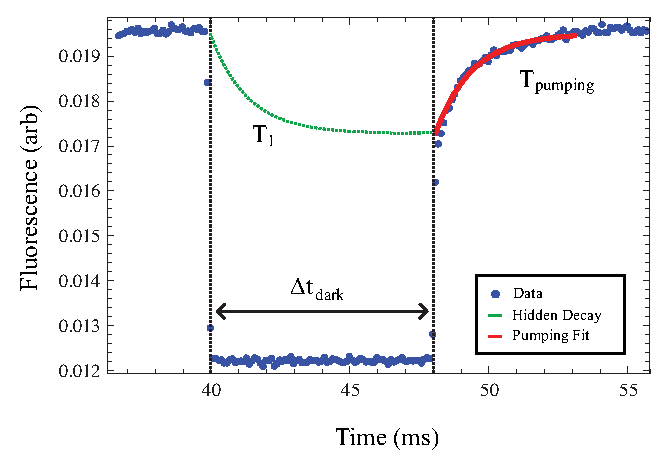
\includegraphics[height=70mm]{./figures/raw_chop.eps}
\caption{\small{Sample data for the $T_1$ and optical pumping time measurement.  An optical chopper blocks the laser lights for some duration $\Delta t$, called the dark time.  During this dark time, the number of atoms in the excited $m_F$ state decreases due to $T_1$ relaxation.  Because the laser is blocked, this decay can only be indirectly measured.  After the dark time, laser light is able to pass through the chopper and optically pump the rubidium atoms.  The red fit is used to determine both the optical pumping time constant and the relative decrease in signal during the dark time. The hidden decay is shown purely for explanatory reasons and is not a fit to the data.}}
\label{fig:chop}
\end{center}
\end{figure}
By setting the optical chopper to different frequencies, we can measure measure the relative decrease in signal for different dark times and thus construct the hidden exponential decay derived in SOMETHING.  Moreover, by fitting the subsequent rise in signal following the unblocking of laser light, we can calculate the optical pumping time constant by fitting to an exponential rise.  Further calculation and analysis of this data is done in Section \ref{DeterminationofTimes}.

\subsection{Measuring Spin Exchange Between $^{85}$Rb and $^{87}$Rb}\label{MeasuringSpinExchange}
By optically pumping $^{85}$Rb and coupling the $m_F$ states of $^{87}$Rb we observe spin exchange between the isotopes. To measure the spin exchange process, we use the lock-in amplifier to measure the amplitude of the Rabi oscillations of $^{85}$Rb atoms which have been excited by the Rabi oscillations of the $^{87}$Rb atoms.  This data is similar to the Lorentzian resonances shown in Fig. \ref{fig:rawcurve}.  This process is repeated while pumping $^{85}$Rb atoms and observing the spin exchange resulting in subsequent Rabi oscilliation of $^{87}$Rb atoms.

In order to determine the natural linewidth of both spin exchange processes we measure the linewidths while varying RF amplitude (this procedure is identical to the one used in Section \ref{MeasuringLinewidthandOpticalPumpingResonance}).  This data is fit to $\alpha \sqrt{1+\beta x^2}$ again using nonlinear regression analysis (shown in Fig. \ref{fig: spinexchange}).
\begin{figure}[htbp]
\begin{center}
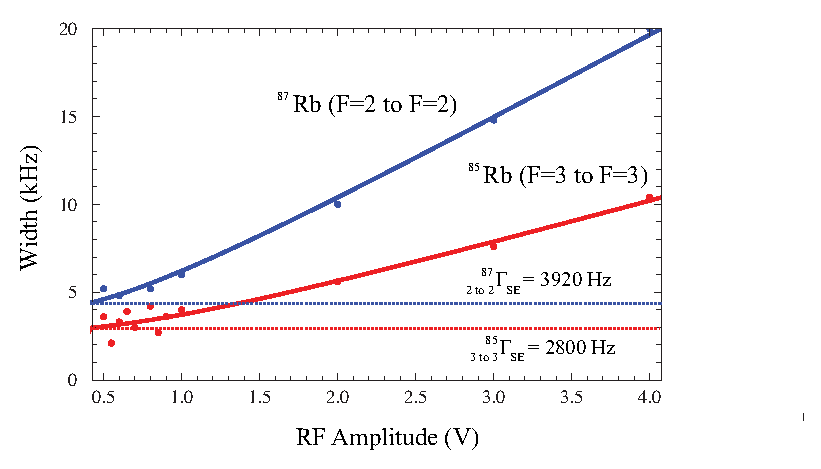
\includegraphics[height=70mm]{./figures/spin_exchange.eps}
\caption{\small{Power broadening of the rubidium spin exchange linewidths due to RF amplitude. By fitting to $\alpha \sqrt{1+\beta x^2}$, we are able to determine the natural spin exchange line widths for $^{85}$Rb and $^{87}$Rb which are found to be $2.80 \pm 0.28$ and kHz $3.92 \pm 0.71$ kHz respectively.  Error is identified by the thickness of the points.}}\label{fig: spinexchange}
\end{center}
\end{figure}
We find the natural linewidths for the spin exchange processes to be $2.80 \pm 0.28$ kHz and $3.92 \pm 0.71$ kHz for $^{85}$Rb and $^{87}$Rb respectively.

%analysis body
%Created MS 05-11

\section{Analysis}\label{analysis}

\subsection{$^{85}$Rb and $^{87}$Rb Spin Analysis}

By measuring the resonant RF frequencies used to induce the coupling of $m_F$ states, we can calculate the $g$-factors for $^{85}$Rb and $^{87}$Rb.  In in Section \ref{linewidth}, we found the resonant frequencies to be $161.7$ kHz for $^{85}$Rb and $243.0$ kHz for $6{87}$Rb.  (values for B, n, I?) Using Equation \ref{BLAH} we calculate $g_F$ for $^{85}$Rb to be $0.30\pm BLAH$ and $g_F$ for $^{87}$Rb to be $0.46\pm BLAH$.  Both calculations are in good agreement with the theoretical values of $1/3$ and $1/2$ respectively. 

Using Equation \ref{eq:BLAH} and our calculated values for $g_F$, we can calculate the nuclear spins of both $^{85}$Rb and $^{87}$Rb in the $^{2}S_{1/2}$ atomic states.  Doing so, we calculate the nuclear spins to be $2.8 \pm BLAH$ and $1.7 \pm BLAH$ respectively.  These calculations are in good agreement with the theoretical values of $5/2$ and $3/2$.

Error Analysis

\subsection{Time Evolution Analysis}

\subsubsection{Determination of $T_{2}$ Relaxation Time}

By measuring the natural linewidth of $^{85}$Rb , we can calculate the $T_2$ relaxation time.  In Section \ref{linewidthmeas}, we found that the natural linewidth of $^{85}$Rb was $370$ kHz.  Using Equation \ref{eq:T2}, we calculate $T2$ to be 


\subsubsection{Determination of the $T_{1}$ Relaxation Time}

\begin{figure}[htbp]
\begin{center}
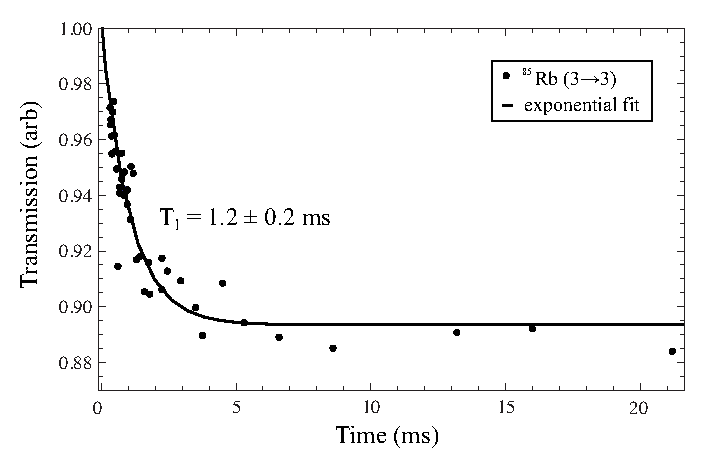
\includegraphics[height=70mm]{./figures/T1.eps}
\caption{\small{}}
\label{fig:}
\end{center}
\end{figure}

\subsubsection{Determination of the Optical Pumping Time}

\subsection{Spin Exchange Analysis}

\subsubsection{Determination of $T_{\mathrm{SE}}$}

\subsubsection{Determination of $\sigma_{\mathrm{SE}}$}

%Conclusion body
%Created MB 04-12

\section{Conclusion}\label{conclusion}

In this experiment, we observe several properties of rubidium atoms in an optical pumping system. We observe Rabi oscillations by pumping atoms to a preferential state $m_{F}$ and coupling them with a radiofrequency signal to a lower $m_{F}$ level. The g-factors for both isotopes of rubidium are calculated to be $g_{F}=0.30\pm0.03$ for $^{85}$Rb and $g_{F}=0.46\pm0.05$ for $^{87}$Rb, within error of the respective expected values $g_{F}=0.33$ and $g_{F}=0.50$. The ratio of g-factors is calculated to be $g_{87}/g_{85}=1.5\pm0.2$, even in stronger agreement with the expected value of $g_{87}/g_{85}=1.5$. The optical pumping time in our experimental conditions was calculated to be $\tau = 5.9\pm 1.5$ ms and the spin relaxation time was found as $T_{1}=1.2 \pm 0.2$ ms, both in reasonable agreement with 


\appendix

\begin{center}
\begin{Large}
\bfseries{Appendices}
\end{Large}
\end{center}


%\addcontentsline{toc}{section}{References}
\newpage
\bibliography{writeup}
\bibliographystyle{abbrv}

\end{document}


